% ===========================================================================
\section{Resultados}
\label{sec:resultados}
% ===========================================================================

Esta se\c{c}\~ao apresenta exclusivamente o que foi obtido: n\'umeros extra\'idos do
relat\'orio de malha, tempos registrados na sess\~ao de refer\^encia, contagens de objetos e
an\'alise comparativa das vistas.

\subsection{Protocolo executado e tempos}

O \emph{build} foi executado dentro de uma sess\~ao viva do Blender, mediada por MCP. A
constru\c{c}\~ao completa da cena leva cerca de 0,6\,s; as nove vistas de
verifica\c{c}\~ao, renderizadas a $1500 \times 1000$ pixels com 64 amostras de
acumula\c{c}\~ao temporal, consomem 45,4\,s no total --- de 3,6\,s (vista superior em
material neutro) a 6,4\,s (detalhe de roda); e a galeria de apresenta\c{c}\~ao, a 96
amostras, consome cerca de 37\,s para cinco imagens. Verificar \'e, portanto, cerca de
setenta e cinco vezes mais caro que reconstruir --- assimetria que justifica investir na
verificabilidade autom\'atica das propriedades estruturais.

\subsection{Resultado do \emph{build}}

A Tabela~\ref{tab:build} consolida os n\'umeros do \'ultimo \emph{build}. Todos os valores
s\~ao reproduz\'iveis por reexecu\c{c}\~ao do \emph{script} e est\~ao registrados no
relat\'orio de malha do projeto.

\begin{table}[htbp]
\centering
\caption{Resumo num\'erico do \emph{build}}
\label{tab:build}
\footnotesize
\begin{tabular}{>{\raggedright\arraybackslash}p{7.2cm}r}
\toprule
\textbf{Grandeza} & \textbf{Valor} \\
\midrule
Objetos de malha & 130 \\
Materiais & 13 \\
Luzes & 4 \\
C\^ameras & 9 \\
Faces (malha base) & 32.632 \\
\quad quads & 29.272 \\
\quad tri\^angulos & 3.360 \\
\quad n-gons & \textbf{0} \\
Arestas n\~ao variedade & \textbf{0} \\
Arestas de borda & 1.776 \\
\bottomrule
\end{tabular}
\fonte{elaborado pelo autor a partir do relat\'orio de malha (2026).}
\end{table}

Dois n\'umeros merecem leitura atenta. O primeiro \'e a contagem de n-gons: zero ---
consequ\^encia direta das decis\~oes de arquitetura (tampa por leque dobrado e
substitui\c{c}\~ao sistem\'atica de tampas n-gon), e n\~ao de uma etapa de limpeza. O
segundo \'e a contagem de arestas de borda: 1.776, todas concentradas nos tr\^es objetos de
emblema, cujos glifos t\^em contorno aberto; nenhum corpo curvo possui aresta de borda. A
decomposi\c{c}\~ao dos 3.360 tri\^angulos mostra que nenhum se encontra em
superf\'icie curva principal: 604 e 252 v\^em dos glifos de \texttt{LOTUS} e
\texttt{111S}, 48 de um canto de chanfro em caixa e os 2.456 restantes de cantos de
chanfro de tr\^es segmentos em primitivas.

\subsection{Integridade topol\'ogica dos corpos principais}

Os dois corpos que definem a superf\'icie vis\'ivel apresentam topologia integralmente
quadrangular: o casco tem 750 quads em 752 v\'ertices, a cabine tem 148 quads em 150
v\'ertices, e ambos t\^em zero n-gons, zero arestas n\~ao variedade e zero arestas de
borda. O arco de seguran\c{c}a (896 quads), o volante (640 quads) e os quatro pneus
($4 \times 720$ quads) tamb\'em s\~ao integralmente quadrangulares. A
verifica\c{c}\~ao aritm\'etica confirma a constru\c{c}\~ao: 47 esta\c{c}\~oes geram 46
faixas de 16 faces (736 quads) e as duas tampas por leque dobrado acrescentam 7 quads
cada, alcan\c{c}ando 750 --- exatamente o valor medido; a cabine segue o mesmo padr\~ao
(14 faixas de 10 faces mais duas tampas de 4 quads = 148). A coincid\^encia entre
c\'alculo e medi\c{c}\~ao \'e a evid\^encia de que a malha \'e exatamente a que o
algoritmo descreve.

\subsection{Envelope dimensional}

A Tabela~\ref{tab:envelope} confronta os valores medidos com os alvos, com toler\^ancia
adotada de $\pm2$\,cm em cada dimens\~ao.

\begin{table}[htbp]
\centering
\caption{Envelope dimensional: alvo, valor medido e desvio}
\label{tab:envelope}
\footnotesize
\begin{tabular}{>{\raggedright\arraybackslash}p{3.6cm}rrr}
\toprule
\textbf{Dimens\~ao} & \textbf{Alvo (m)} & \textbf{Medido (m)} & \textbf{Desvio (cm)} \\
\midrule
Comprimento (X) & 3,726 & 3,736 & $+1,0$ \\
Largura (Y) & 1,718 & 1,718 & $0,0$ \\
Altura (Z) & 1,117 & 1,117 & $0,0$ \\
\bottomrule
\end{tabular}
\fonte{elaborado pelo autor a partir do relat\'orio de malha (2026); solo em
$Z = 0{,}0000$\,m e centro em $Y = 0{,}0000$\,m.}
\end{table}

O \'unico desvio \'e de $+1,0$\,cm no comprimento, atribu\'ivel \`as tampas de
extremidade: a tampa por leque dobrado \'e uma superf\'icie n\~ao plana que avan\c{c}a
ligeiramente al\'em do plano da \'ultima esta\c{c}\~ao, mas permanece dentro da
toler\^ancia. A largura e a altura s\~ao exatas porque a largura m\'axima e a cota do topo
s\~ao par\^ametros diretos das esta\c{c}\~oes, e n\~ao grandezas emergentes.

\subsection{Conte\'udo da cena}

As rodas, sozinhas, respondem por 52 dos 130 objetos de malha (quarenta por cento da
cena), refletindo seu n\'umero de partes reais: aro, disco, cubo, tampa, seis raios,
pneu, disco de freio e pin\c{c}a. Seguem-se ventila\c{c}\~oes (23), far\'ois e indicadores
(12), lanternas traseiras (8), interior (7), grelha frontal (6), aerodin\^amica (6),
far\'ois auxiliares e espelhos (4 cada), casco, cabine e emblemas (3 cada) e refletores do
difusor (2).

\subsection{An\'alise visual comparativa}

As figuras a seguir justap\~oem refer\^encia e render na mesma escala relativa. Na vista
\textbf{frontal}, os dois far\'ois ovais, a grelha central rebaixada e os dois far\'ois
auxiliares redondos coincidem em posi\c{c}\~ao relativa, e a linha do cap\^o apresenta a
inflex\~ao descendente caracter\'istica sobre cada para-lama (CA-005 atendido). Na vista
\textbf{traseira}, est\~ao presentes as quatro lanternas redondas com aro met\'alico, os
emblemas \texttt{LOTUS} e \texttt{111S} como malha tridimensional, o difusor com duas
sa\'idas de escape centrais e os dois refletores (CA-006 e CA-009 atendidos); em
amplia\c{c}\~ao, a superf\'icie do texto \texttt{LOTUS} apresenta facetas nos cantos dos
glifos, efeito n\~ao percept\'ivel na escala normal de observa\c{c}\~ao.

\begin{figure}[htbp]
  \centering
  \begin{tabular}{cc}
    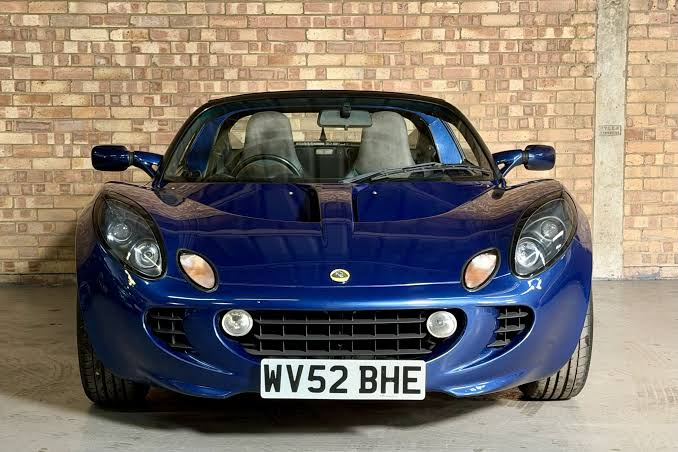
\includegraphics[height=2.3cm]{figures/ref-frontal.jpeg} &
    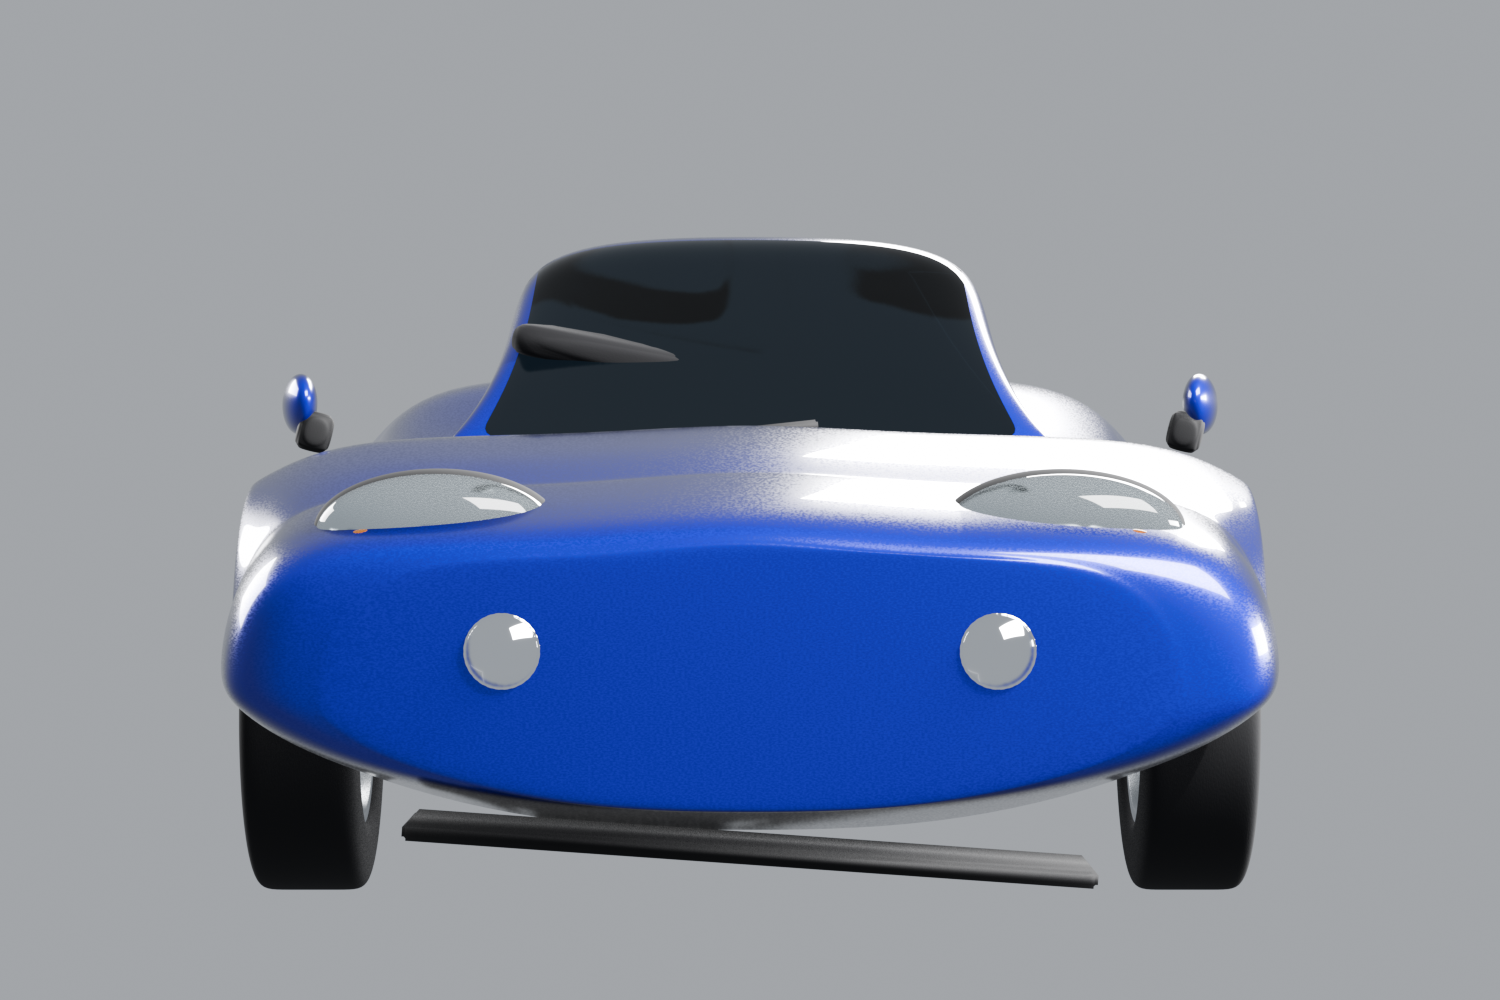
\includegraphics[height=2.3cm]{figures/ver-frontal.png} \\
    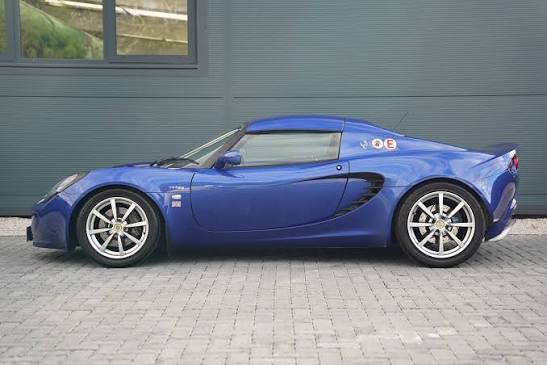
\includegraphics[height=2.3cm]{figures/ref-lateral.jpeg} &
    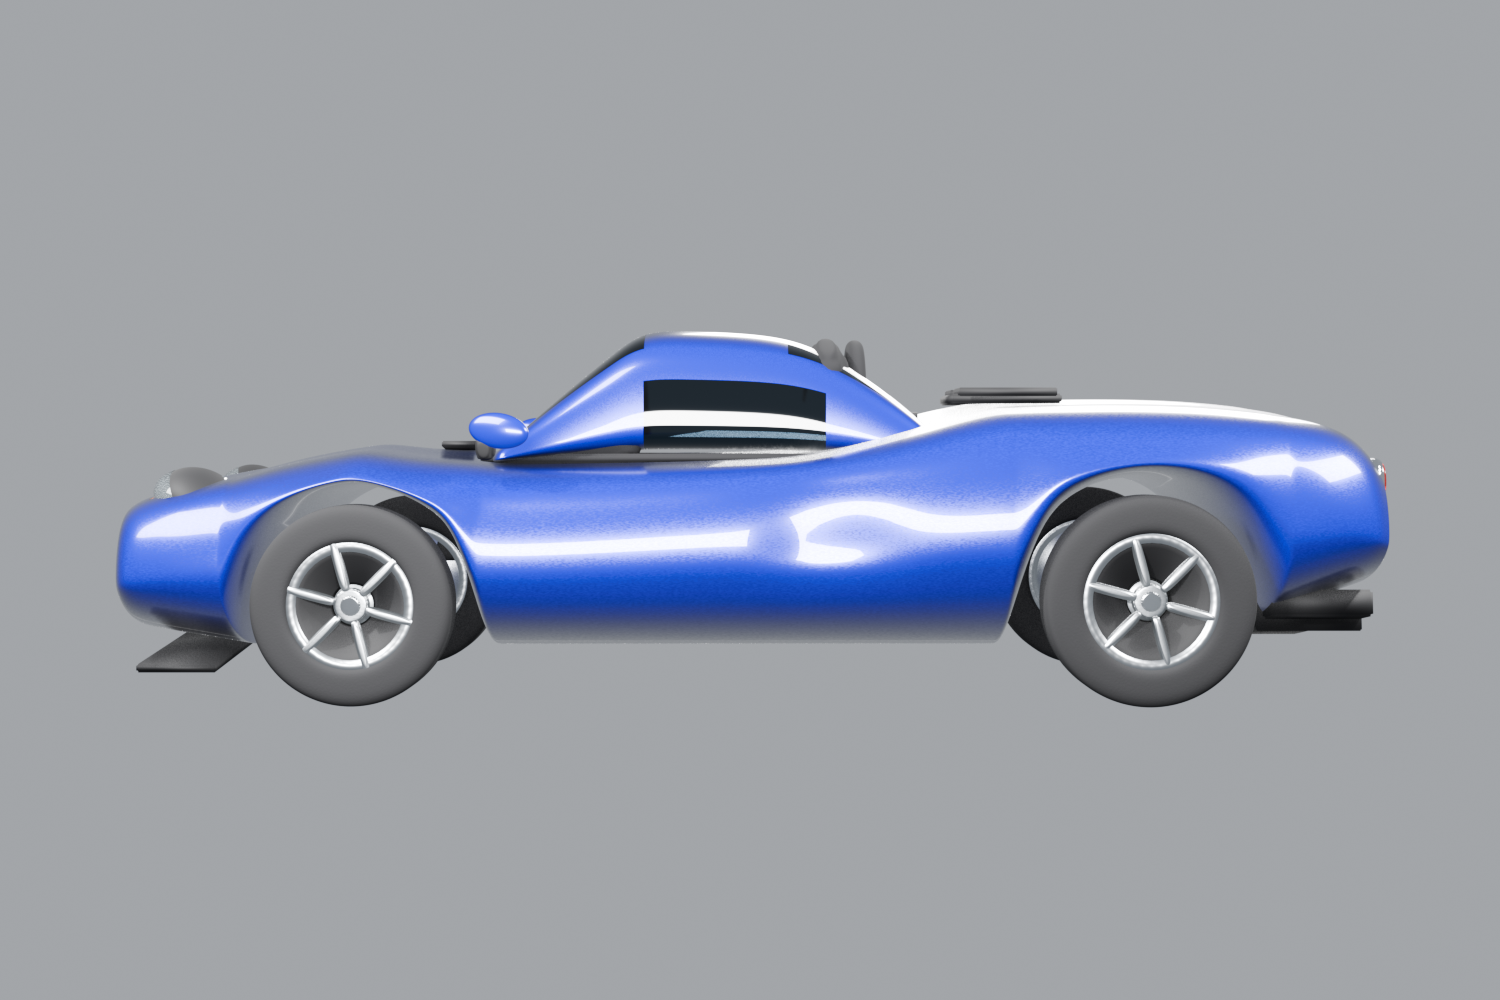
\includegraphics[height=2.3cm]{figures/ver-lateral.png} \\
    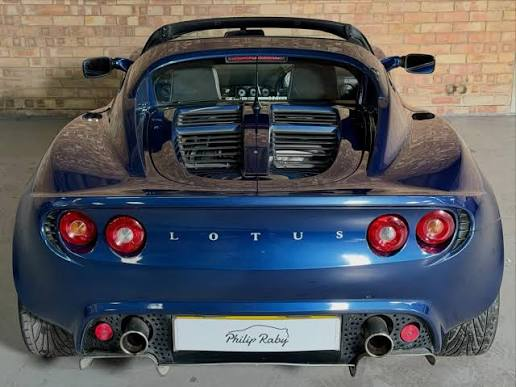
\includegraphics[height=2.3cm]{figures/ref-traseira1.jpeg} &
    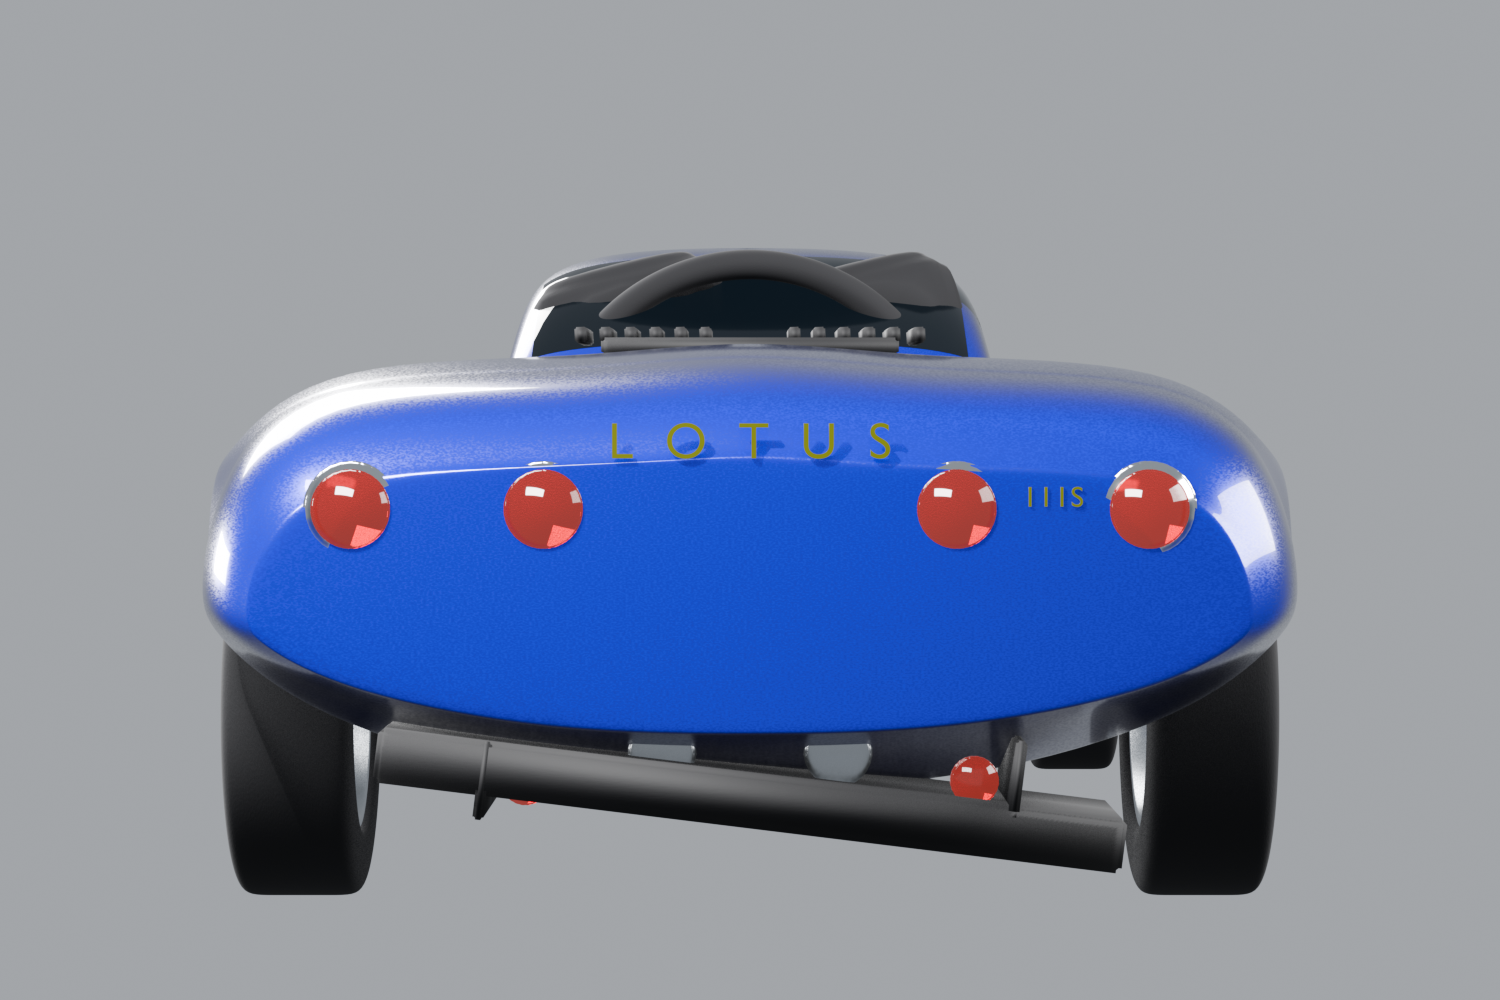
\includegraphics[height=2.3cm]{figures/ver-traseira.png}
  \end{tabular}
  \caption{Vistas frontal (topo), lateral (centro) e traseira (base): refer\^encia \`a
           esquerda e render \`a direita.}
  \label{fig:cmp-a}
  \fonte{acervo do projeto e render pr\'oprio (2026).}
\end{figure}

A vista \textbf{lateral} \'e a mais informativa e a que exp\~oe a limita\c{c}\~ao mais
relevante do resultado. As propor\c{c}\~oes gerais --- altura da cintura,
posi\c{c}\~ao dos eixos, rela\c{c}\~ao entre o comprimento do cap\^o e o da traseira, arco
de roda proeminente --- s\~ao coerentes com a refer\^encia, e o nariz baixo e a cauda
truncada est\~ao presentes. O desvio identificado \'e de outra natureza: falta \`a
superf\'icie a \emph{linha de car\'ater} lateral, a curva de raio pequeno que atravessa a
lateral do ve\'iculo e que, na refer\^encia, produz uma quebra deliberada nos reflexos. No
modelo, essa regi\~ao \'e suave, porque a subdivis\~ao suaviza qualquer varia\c{c}\~ao que
n\~ao esteja sustentada por um anel de proximidade; o corpo fica ligeiramente mais
arredondado que o real, e por isso CA-004 \'e \textbf{parcial}.

A vista \textbf{superior} revela as entradas de ar laterais atr\'as das portas, os
\emph{louvres} do \emph{engine cover}, a posi\c{c}\~ao relativa da cabine e o arco de
seguran\c{c}a (CA-008 atendido). Na vista em \textbf{tr\^es-quartos}, com a refer\^encia de
mesma cor do material, os reflexos s\~ao cont\'inuos ao longo do para-lama dianteiro e da
lateral, sem facetas ou ondula\c{c}\~oes vis\'iveis, o que confirma a integridade da
superf\'icie; o tom, por\'em, ficou ligeiramente mais escuro que a refer\^encia. Duas causas
concorrem: a exposi\c{c}\~ao global foi reduzida ($-0{,}18$) para preservar as altas luzes
nos reflexos especulares, e a refer\^encia passou pelo mapeamento de tons da c\^amera,
diferente do AgX. Isolar a contribui\c{c}\~ao de cada causa exigiria um experimento
controlado com alvo de cor f\'isico, que n\~ao foi realizado (CA-007 \textbf{parcial}).

\begin{figure}[htbp]
  \centering
  \begin{tabular}{cc}
    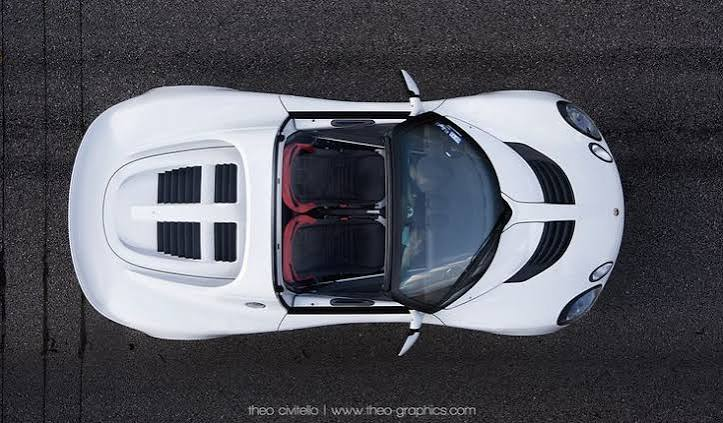
\includegraphics[height=2.6cm]{figures/ref-superior.jpeg} &
    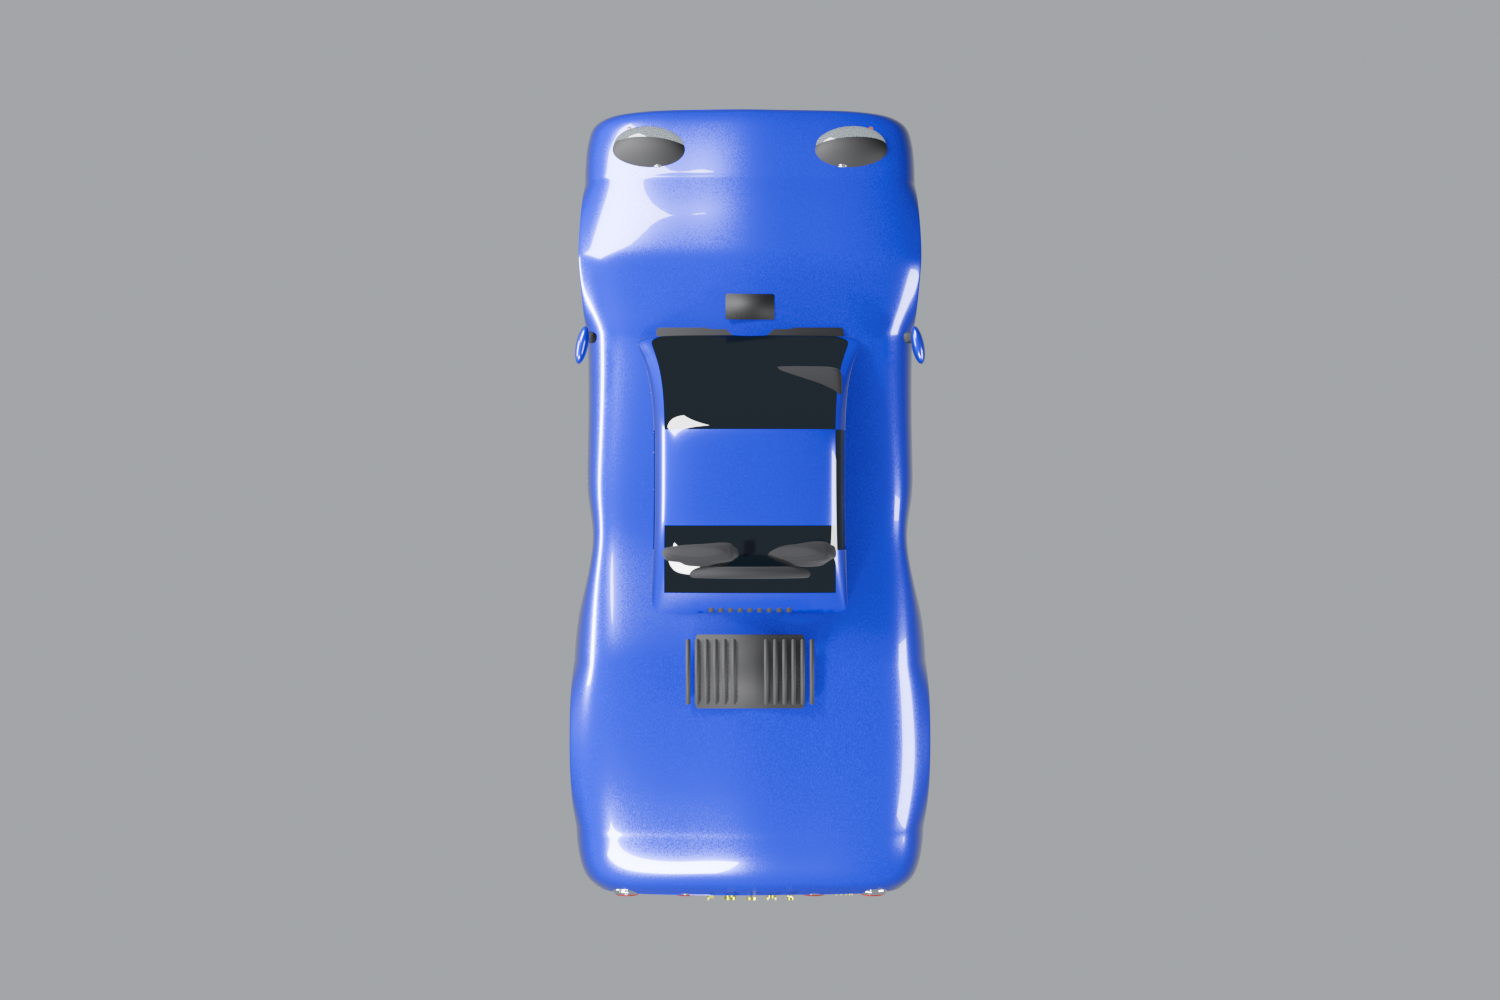
\includegraphics[height=2.6cm]{figures/ver-superior.png} \\
    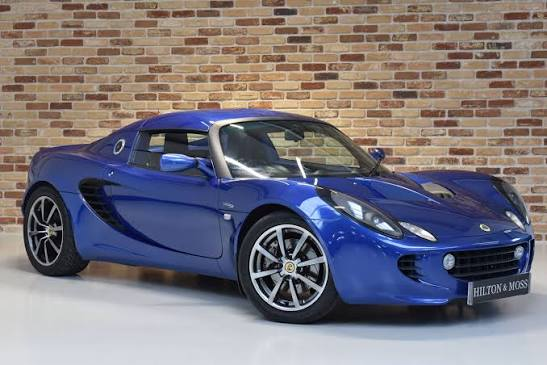
\includegraphics[height=2.6cm]{figures/ref-car.jpeg} &
    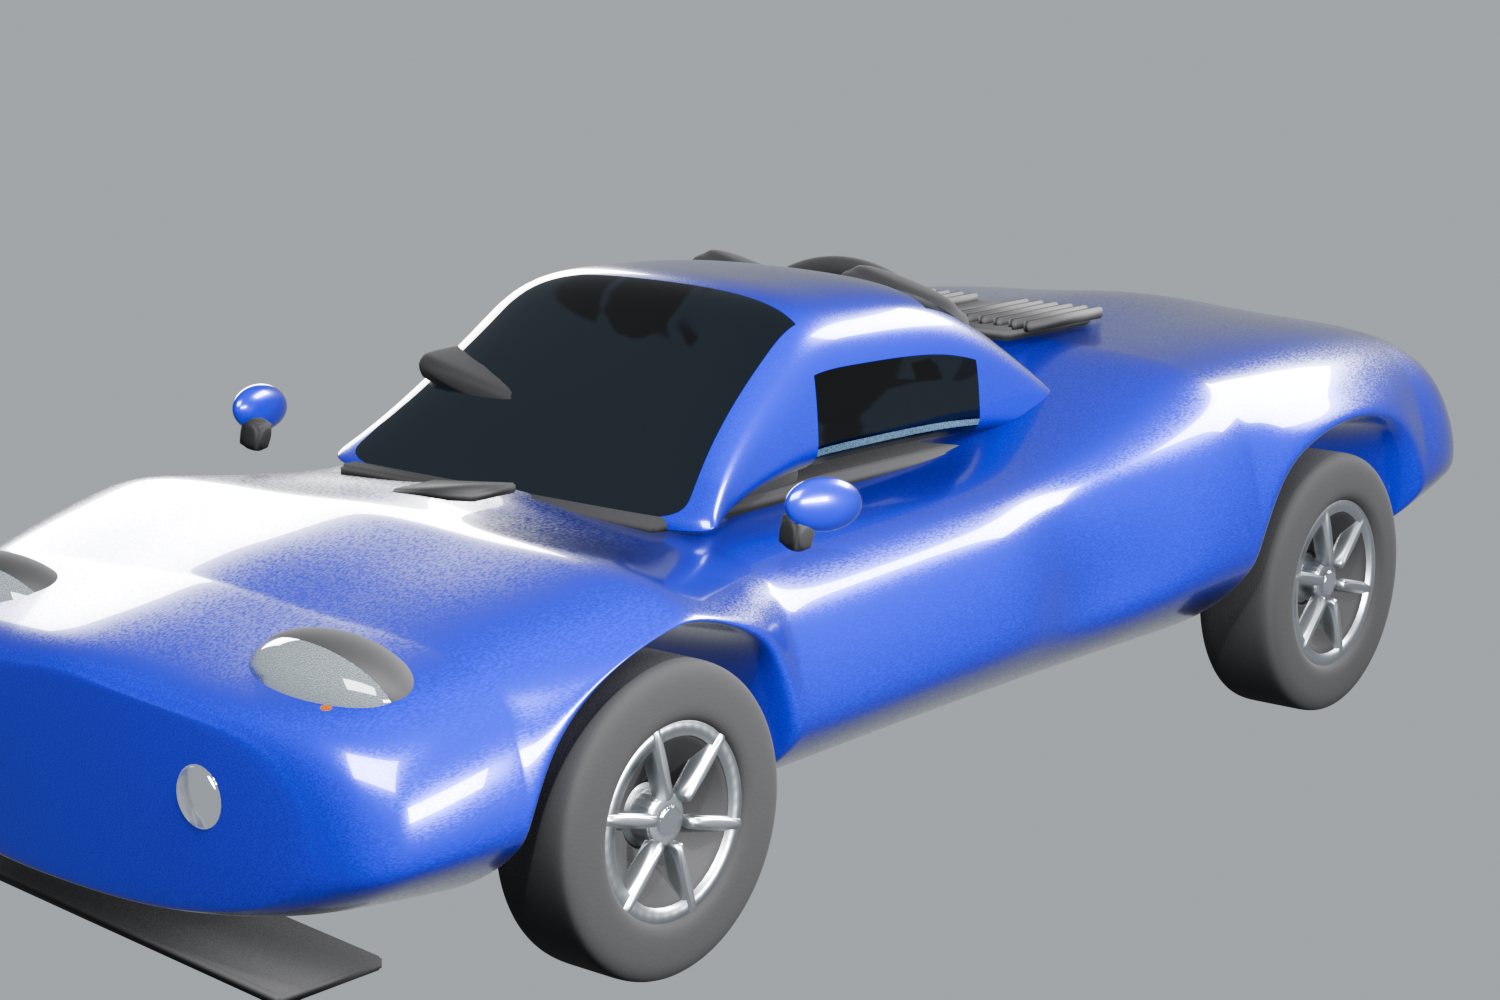
\includegraphics[height=2.6cm]{figures/ver-3q.png}
  \end{tabular}
  \caption{Vistas superior (topo) e em tr\^es-quartos (base): refer\^encia \`a esquerda e
           render \`a direita.}
  \label{fig:cmp-b}
  \fonte{acervo do projeto e render pr\'oprio (2026).}
\end{figure}

O \emph{close} da roda dianteira mostra os seis raios distintos, com tampa central, disco e
pin\c{c}a de freio; o pneu apresenta perfil e propor\c{c}\~ao derivados da
designa\c{c}\~ao 185/55R15. A vista lateral em material neutro remove a vari\'avel da cor e
do verniz e \'e a evid\^encia mais clara da limita\c{c}\~ao de silhueta: sem o verniz, a
superf\'icie \'e uniformemente suave, e a aus\^encia da aresta viva ao longo do para-lama
torna-se evidente.

\begin{figure}[htbp]
  \centering
  \begin{tabular}{cc}
    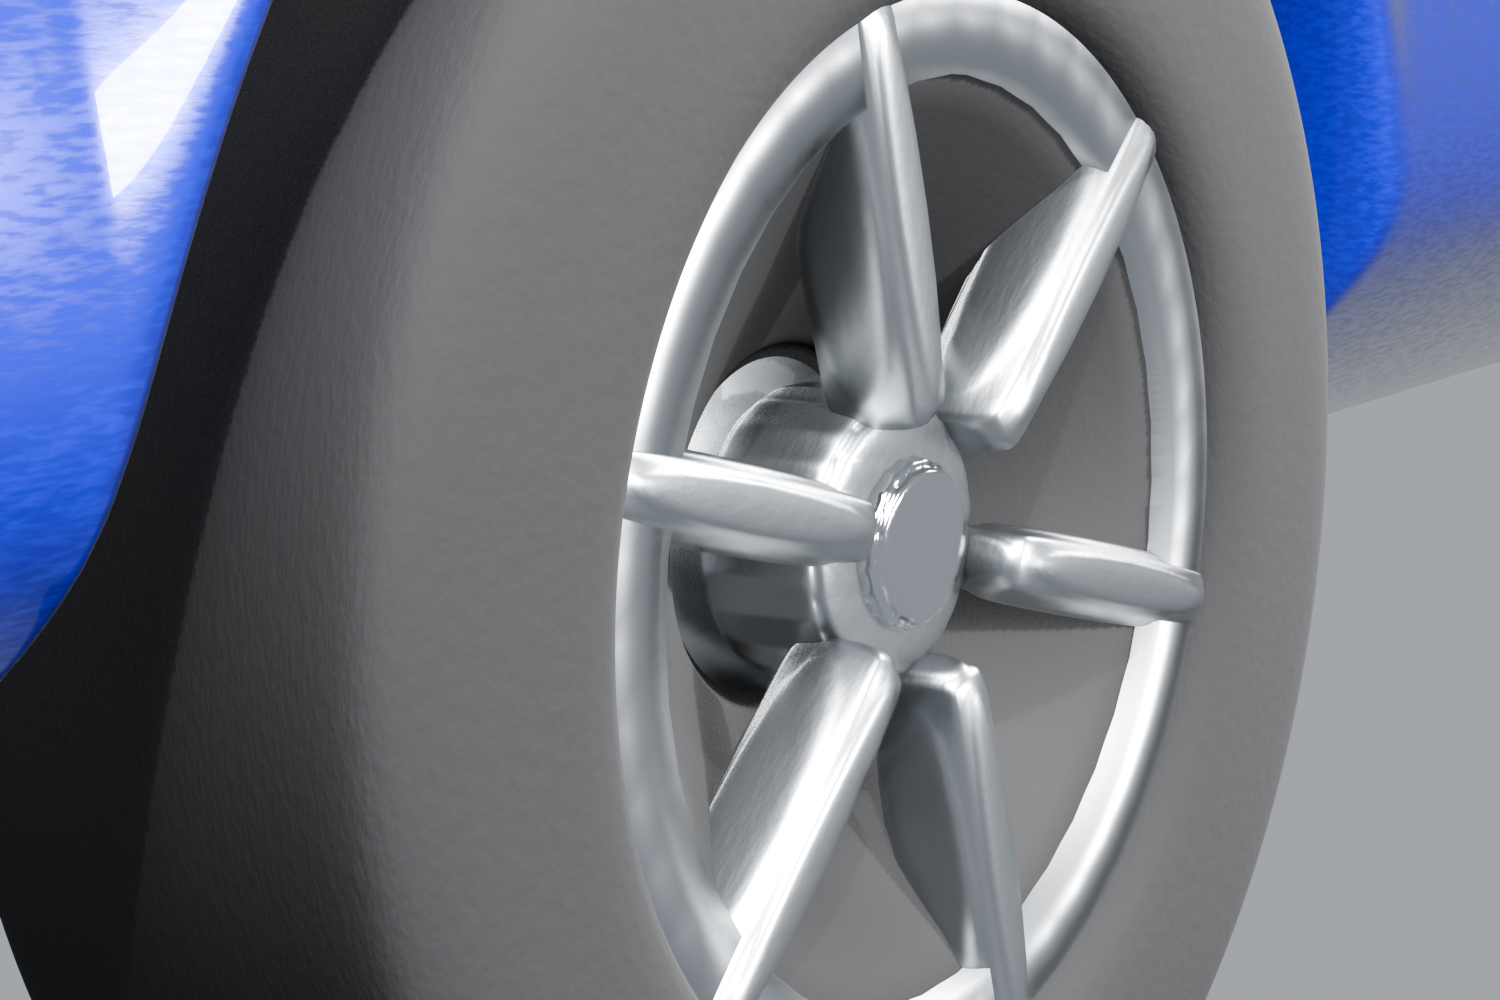
\includegraphics[height=3.4cm]{figures/ver-roda.png} &
    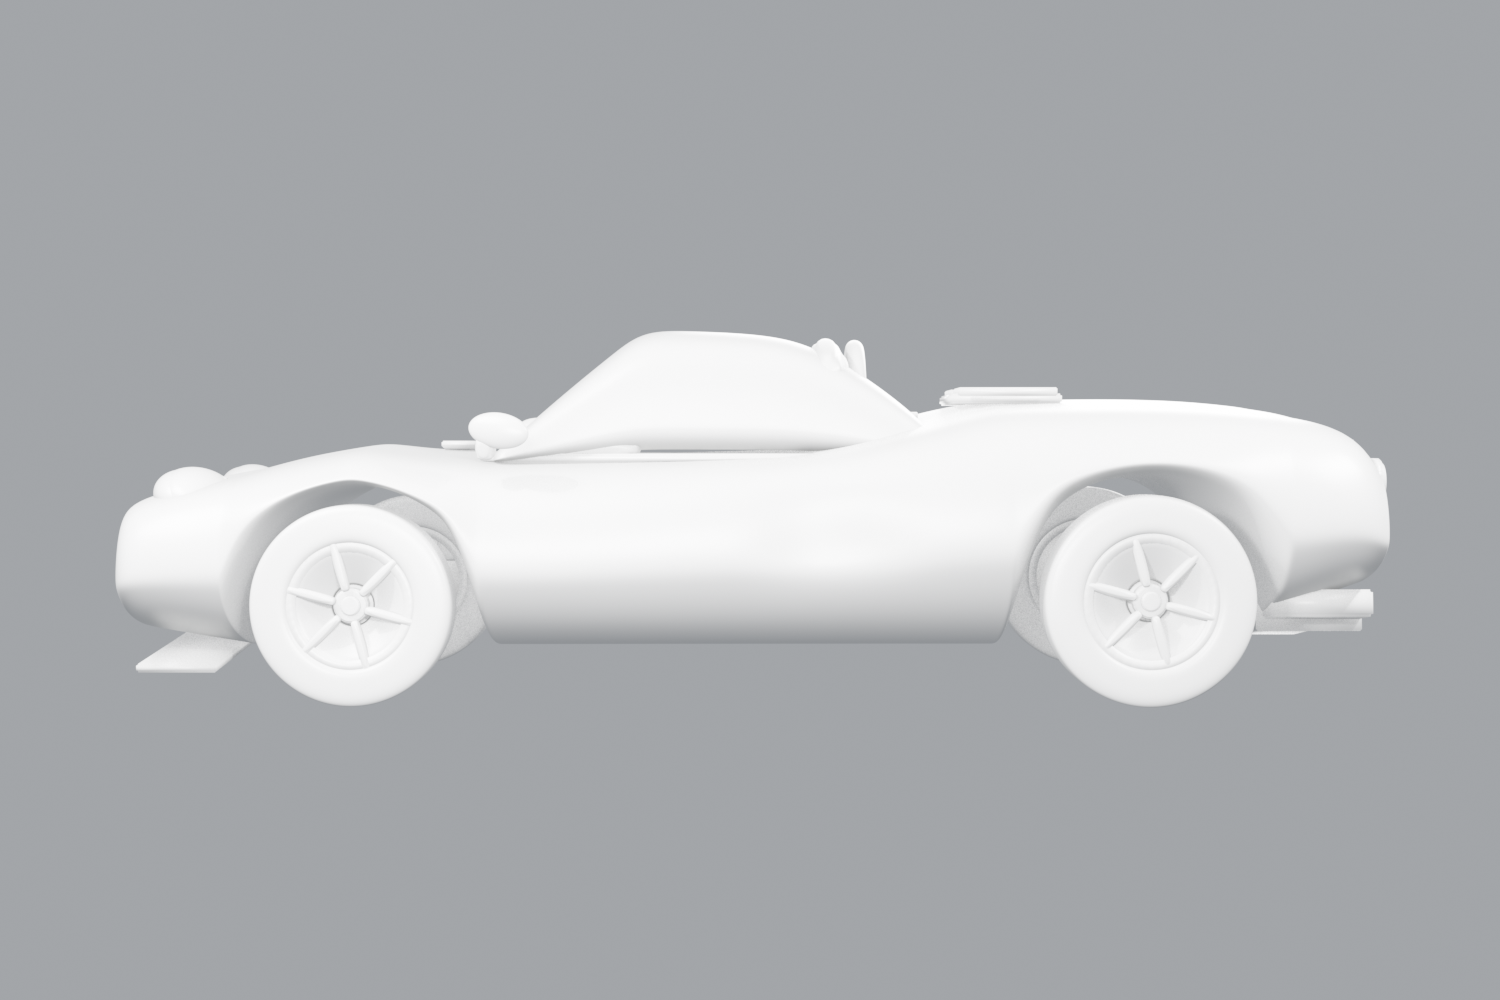
\includegraphics[height=3.4cm]{figures/ver-clay-lateral.png}
  \end{tabular}
  \caption{\`A esquerda, detalhe da roda dianteira (seis raios, tampa central, disco e
           pin\c{c}a); \`a direita, vista lateral em material neutro.}
  \label{fig:roda-clay}
  \fonte{elaborado pelo autor (2026).}
\end{figure}

\subsection{Resultado por crit\'erio de aceita\c{c}\~ao}

A Tabela~\ref{tab:crit} consolida os crit\'erios, o m\'etodo de verifica\c{c}\~ao
aplicado, o status e a evid\^encia. Sete dos nove crit\'erios foram plenamente atendidos;
dois ficaram parciais.

\begin{table}[htbp]
\centering
\caption{Crit\'erios de aceita\c{c}\~ao, m\'etodo de verifica\c{c}\~ao, status e evid\^encia}
\label{tab:crit}
\footnotesize
\begin{tabular}{>{\raggedright\arraybackslash}p{1.0cm}>{\raggedright\arraybackslash}p{3.9cm}>{\raggedright\arraybackslash}p{2.9cm}>{\raggedright\arraybackslash}p{1.75cm}>{\raggedright\arraybackslash}p{3.85cm}}
\toprule
\textbf{ID} & \textbf{Crit\'erio} & \textbf{M\'etodo} & \textbf{Status} & \textbf{Evid\^encia} \\
\midrule
CA-001 & \emph{Build} reconstr\'oi o modelo sem erro & execu\c{c}\~ao do \emph{script} & PASS & 130 objetos \texttt{GEO\_*} \\
CA-002 & Envelope dentro de $\pm2$\,cm dos alvos & medi\c{c}\~ao num\'erica & PASS & $+1{,}0$\,cm em X; Y e Z exatos \\
CA-003 & Zero n-gons e normais coerentes nos corpos & relat\'orio de malha & PASS & 0 n-gons; 0 n\~ao variedade \\
CA-004 & Silhueta lateral coerente com a refer\^encia & inspe\c{c}\~ao visual & \textbf{PARCIAL} & falta a linha de car\'ater (Fig.~\ref{fig:cmp-a}) \\
CA-005 & Frente com far\'ois ovais, grelha e auxiliares & inspe\c{c}\~ao visual & PASS & Fig.~\ref{fig:cmp-a} \\
CA-006 & Traseira com lanternas, \emph{lettering}, escapes e difusor & inspe\c{c}\~ao visual & PASS & Fig.~\ref{fig:cmp-a} \\
CA-007 & Pintura com reflexos cont\'inuos, sem facetas & inspe\c{c}\~ao visual & \textbf{PARCIAL} & tom mais escuro (Fig.~\ref{fig:cmp-b}) \\
CA-008 & Vista superior com entradas de ar, \emph{louvres} e arco & inspe\c{c}\~ao visual & PASS & Fig.~\ref{fig:cmp-b} \\
CA-009 & Nomenclatura e metadados em todos os objetos & inspe\c{c}\~ao do arquivo & PASS & \texttt{cat}, \texttt{part}, \texttt{mat\_swap\_key} \\
\bottomrule
\end{tabular}
\fonte{elaborado pelo autor (2026).}
\end{table}

\subsection{S\'intese dos resultados}

Os resultados sustentam quatro afirma\c{c}\~oes verific\'aveis: a geometria \'e
integralmente quadrangular nos corpos principais, com zero n-gons e zero arestas n\~ao
variedade em toda a cena; o envelope atende \`a toler\^ancia, com desvio m\'aximo de
$1{,}0$\,cm; os elementos de identidade da variante --- rodas de seis raios, conjunto
\'optico, entradas de ar com geometria real, emblemas --- est\~ao presentes e s\~ao
verific\'aveis nos renders; e a fidelidade de silhueta e de tom \'e parcial, com causas
identificadas e localizadas. A aus\^encia de um controle experimental --- um segundo
modelo constru\'ido pelo m\'etodo manual --- impede que se afirme, com base em
medi\c{c}\~ao, que este \emph{pipeline} seja melhor que o tradicional; o que se pode
afirmar \'e que o artefato \'e reconstru\'ivel por um comando, que suas propriedades
estruturais s\~ao medidas automaticamente e que cada decis\~ao geom\'etrica \'e
rastre\'avel at\'e uma linha de c\'odigo.
